%% BioMed_Central_Tex_Template_v1.06
%%                                      %
%  bmc_article.tex            ver: 1.06 %
%                                       %

%%IMPORTANT: do not delete the first line of this template
%%It must be present to enable the BMC Submission system to
%%recognise this template!!

%%%%%%%%%%%%%%%%%%%%%%%%%%%%%%%%%%%%%%%%%
%%                                     %%
%%  LaTeX template for BioMed Central  %%
%%     journal article submissions     %%
%%                                     %%
%%          <8 June 2012>              %%
%%                                     %%
%%                                     %%
%%%%%%%%%%%%%%%%%%%%%%%%%%%%%%%%%%%%%%%%%


%%%%%%%%%%%%%%%%%%%%%%%%%%%%%%%%%%%%%%%%%%%%%%%%%%%%%%%%%%%%%%%%%%%%%
%%                                                                 %%
%% For instructions on how to fill out this Tex template           %%
%% document please refer to Readme.html and the instructions for   %%
%% authors page on the biomed central website                      %%
%% http://www.biomedcentral.com/info/authors/                      %%
%%                                                                 %%
%% Please do not use \input{...} to include other tex files.       %%
%% Submit your LaTeX manuscript as one .tex document.              %%
%%                                                                 %%
%% All additional figures and files should be attached             %%
%% separately and not embedded in the \TeX\ document itself.       %%
%%                                                                 %%
%% BioMed Central currently use the MikTex distribution of         %%
%% TeX for Windows) of TeX and LaTeX.  This is available from      %%
%% http://www.miktex.org                                           %%
%%                                                                 %%
%%%%%%%%%%%%%%%%%%%%%%%%%%%%%%%%%%%%%%%%%%%%%%%%%%%%%%%%%%%%%%%%%%%%%

%%% additional documentclass options:
% \documentclass[doublespacing]
% [linenumbers]   - put the line numbers on margins

%%% loading packages, author definitions

%\documentclass[twocolumn]{bmcart}% uncomment this for twocolumn layout and comment line below
\documentclass[doublespacing, linenumbers]{bmcart}



%%% Load packages
%\usepackage{amsthm,amsmath}
%\RequirePackage{natbib}
\RequirePackage{hyperref}
\usepackage[utf8]{inputenc} %unicode support
\usepackage{lscape}
\usepackage{graphicx}
\usepackage{pdflscape}
%\usepackage[applemac]{inputenc} %applemac support if unicode package fails
%\usepackage[latin1]{inputenc} %UNIX support if unicode package fails


%%%%%%%%%%%%%%%%%%%%%%%%%%%%%%%%%%%%%%%%%%%%%%%%%
%%                                             %%
%%  If you wish to display your graphics for   %%
%%  your own use using includegraphic or       %%
%%  includegraphics, then comment out the      %%
%%  following two lines of code.               %%
%%  NB: These line *must* be included when     %%
%%  submitting to BMC.                         %%
%%  All figure files must be submitted as      %%
%%  separate graphics through the BMC          %%
%%  submission process, not included in the    %%
%%  submitted article.                         %%
%%                                             %%
%%%%%%%%%%%%%%%%%%%%%%%%%%%%%%%%%%%%%%%%%%%%%%%%%


% \def\includegraphic{}
% \def\includegraphics{}



%%% Put your definitions there:
\startlocaldefs
\endlocaldefs


%%% Begin ...
\begin{document}

%%% Start of article front matter
\begin{frontmatter}

\begin{fmbox}
\dochead{Research}

%%%%%%%%%%%%%%%%%%%%%%%%%%%%%%%%%%%%%%%%%%%%%%
%%                                          %%
%% Enter the title of your article here     %%
%%                                          %%
%%%%%%%%%%%%%%%%%%%%%%%%%%%%%%%%%%%%%%%%%%%%%%

\title{SuperPhy: Predictive genomics for priority food-borne pathogens}

%%%%%%%%%%%%%%%%%%%%%%%%%%%%%%%%%%%%%%%%%%%%%%
%%                                          %%
%% Enter the authors here                   %%
%%                                          %%
%% Specify information, if available,       %%
%% in the form:                             %%
%%   <key>={<id1>,<id2>}                    %%
%%   <key>=                                 %%
%% Comment or delete the keys which are     %%
%% not used. Repeat \author command as much %%
%% as required.                             %%
%%                                          %%
%%%%%%%%%%%%%%%%%%%%%%%%%%%%%%%%%%%%%%%%%%%%%%

\author[
   addressref={aff1},                   % id's of addresses, e.g. {aff1,aff2}                      % id of corresponding address, if any
   noteref={n1},                        % id's of article notes, if any
   email={matthew.whiteside@phac-aspc.gc.ca}   % email address
]{\inits{MD}\fnm{Matthew D} \snm{Whiteside}}
\author[
   addressref={aff1},
   email={chad.r.laing@phac-aspc.gc.ca},
   noteref={n1}
]{\inits{CR}\fnm{Chad R} \snm{Laing}}
\author[
  addressref={aff1},
  email={akiff.manji@phac-aspc.gc.ca}
]{\inits{A}\fnm{Akiff} \snm{Manji}}
\author[
  addressref={aff1},
  email={peter.kruczkiewicz@phac-aspc.gc.ca}
]{\inits{P}\fnm{Peter} \snm{Kruczkiewicz}}
\author[
  addressref={aff1},
  email={eduardo.taboada@phac-aspc.gc.ca}
]{\inits{EN}\fnm{Eduardo N} \snm{Taboada}}
\author[
  addressref={aff1},
  email={vic.gannon@phac-aspc.gc.ca},
  corref={aff1}, 
]{\inits{VPJ}\fnm{Victor PJ} \snm{Gannon}}


%%%%%%%%%%%%%%%%%%%%%%%%%%%%%%%%%%%%%%%%%%%%%%
%%                                          %%
%% Enter the authors' addresses here        %%
%%                                          %%
%% Repeat \address commands as much as      %%
%% required.                                %%
%%                                          %%
%%%%%%%%%%%%%%%%%%%%%%%%%%%%%%%%%%%%%%%%%%%%%%

\address[id=aff1]{%                           % unique id
  \orgname{Laboratory for Foodborne Zoonoses, Public Health Agency of Canada}, % university, etc
  \street{Twp Rd 9-1},                     %
  \postcode{T1J 3Z4}                                % post or zip code
  \city{Lethbridge},                              % city
  \cny{Canada}                                    % country
}

%%%%%%%%%%%%%%%%%%%%%%%%%%%%%%%%%%%%%%%%%%%%%%
%%                                          %%
%% Enter short notes here                   %%
%%                                          %%
%% Short notes will be after addresses      %%
%% on first page.                           %%
%%                                          %%
%%%%%%%%%%%%%%%%%%%%%%%%%%%%%%%%%%%%%%%%%%%%%%

\begin{artnotes}
%\note{Sample of title note}     % note to the article
\note[id=n1]{Equal contributor} % note, connected to author
\end{artnotes}

\end{fmbox}% comment this for two column layout

%%%%%%%%%%%%%%%%%%%%%%%%%%%%%%%%%%%%%%%%%%%%%%
%%                                          %%
%% The Abstract begins here                 %%
%%                                          %%
%% Please refer to the Instructions for     %%
%% authors on http://www.biomedcentral.com  %%
%% and include the section headings         %%
%% accordingly for your article type.       %%
%%                                          %%
%%%%%%%%%%%%%%%%%%%%%%%%%%%%%%%%%%%%%%%%%%%%%%

\begin{abstractbox}

\begin{abstract} % abstract
% \parttitle{First part title} %if any
% \parttitle{Second part title} %if any

Predictive genomics involves the translation of raw genome sequence data into an assessment of the phenotypes exhibited by the organism. For bacterial pathogens, these phenotypes can range from survivability in hostile environmental conditions, to whether an organism can cause severe human disease. Significant progress has been made in the development of generic tools for genomic analyses that are broadly applicable to all microorganisms; however, a fundamental missing component is the ability to analyze genomic data in the context of organism-specific knowledge, which has been accumulated from decades of research and can provide a meaningful interpretation for the data. 

In this study, we present SuperPhy, an online predictive genomics platform \url{http://lfz.corefacility.ca/superphy/} for \textit{Escherichia coli}. The platform integrates the analyses tools and genome sequence data for all publicly available \textit{E. coli} genomes and facilitates the upload of new genome sequences from users under public or private settings. SuperPhy provides real-time analyses of thousands of genome sequences with results that are understandable and useful to a wide community, including those in the fields of clinical medicine, epidemiology, ecology, and evolution. SuperPhy includes identification of: 1) virulence and antimicrobial resistance determinants 2) epidemiological associations between specific genotypes, biomarkers, geospatial distribution, host, source, and other metaadata 3) statistically significant genome markers (presence / absence of specific genomic regions, and single-nucleotide polymorphisms) based on phylogenetic clade, and 4) \textit{in silico} Shiga-toxin subtyping. 

SuperPhy allows researchers to quickly analyze and compare new genomes with all other publicly available sequenced \textit{E. coli} strains. Predictive genomics provides an essential link between the vast amounts of genome information currently being generated and biological knowledge in an organism-specific context. 

\end{abstract}

%%%%%%%%%%%%%%%%%%%%%%%%%%%%%%%%%%%%%%%%%%%%%%
%%                                          %%
%% The keywords begin here                  %%
%%                                          %%
%% Put each keyword in separate \kwd{}.     %%
%%                                          %%
%%%%%%%%%%%%%%%%%%%%%%%%%%%%%%%%%%%%%%%%%%%%%%

\begin{keyword}
\kwd{sample}
\kwd{article}
\kwd{author}
\end{keyword}

% MSC classifications codes, if any
%\begin{keyword}[class=AMS]
%\kwd[Primary ]{}
%\kwd{}
%\kwd[; secondary ]{}
%\end{keyword}

\end{abstractbox}
%
%\end{fmbox}% uncomment this for twcolumn layout
\end{frontmatter}

%%%%%%%%%%%%%%%%%%%%%%%%%%%%%%%%%%%%%%%%%%%%%%
%%                                          %%
%% The Main Body begins here                %%
%%                                          %%
%% Please refer to the instructions for     %%
%% authors on:                              %%
%% http://www.biomedcentral.com/info/authors%%
%% and include the section headings         %%
%% accordingly for your article type.       %%
%%                                          %%
%% See the Results and Discussion section   %%
%% for details on how to create sub-sections%%
%%                                          %%
%% use \cite{...} to cite references        %%
%%  \cite{koon} and                         %%
%%  \cite{oreg,khar,zvai,xjon,schn,pond}    %%
%%  \nocite{smith,marg,hunn,advi,koha,mouse}%%
%%                                          %%
%%%%%%%%%%%%%%%%%%%%%%%%%%%%%%%%%%%%%%%%%%%%%%

%%%%%%%%%%%%%%%%%%%%%%%%% start of article main body
% <put your article body there>

%%%%%%%%%%%%%%%%
%% Background %%
%%
\section*{Introduction}
Whole-genome sequencing (WGS) of bacterial isolates generates the complete DNA sequence of each organism. WGS provides the most possible resolution of any typing method, the sequence is easily transferable, and an analysis of its contents can reveal important phenotypic insights such as the presence of virulence factors or anti-microbial resistance determinants. Current benchtop platforms such as the Illumina MiSeq and the newly developed USB-sized Oxford Nanopore sequencer have hastened a change where real-time WGS can be performed in the laboratory as well as on the front-line, as was recently seen in the 2014 Ebola outbreak, and in managing a hospital outbreak of \textit{Salmonella} \cite{jones_technology:_2015,gilchrist_whole-genome_2015,birmingham_how_2015,quick_rapid_2015}. 

WGS can be used in real-time, without the cost in time and supplies of wet-lab methods, in identifying the source of foodborne outbreaks \cite{graham_real-time_2014}, surveillance \cite{zankari_genotyping_2013,cody_real-time_2013},  epidemiological investigations \cite{cody_real-time_2013}, industry \cite{andreevskaya_genome_2015,mazzaglia_pseudomonas_2012}, population studies \cite{nasser_evolutionary_2014,kopac_genomic_2014}, routine typing \cite{zhang_salmonella_2015}, regulation \cite{halachev_genomic_2014}, policy formation , providing on-site insight to clinicians \cite{grad_epidemiologic_2014,jr_next-generation_2012}, informing veterinary practice \cite{biek_whole_2012}, and helping inform public-health decisions \cite{lemke_stakeholder_2015}.

  WGS is now the \textit{de facto} standard for bacterial analyses and the global community is coming together to help store and best utilize this rapid influx of information under the Global Microbial Identifier network \url{(http://www.globalmicrobialidentifier.org/}. This international effort currently incorporates 32 countries, many of which have their own national or regional programs to best utilize WGS data in public health, epidemiological and research contexts, such as the GenomeTrakR initiative of the Food and Drug Administration in the United States of America \url{http://www.fda.gov/Food/FoodScienceResearch/WholeGenomeSequencingProgramWGS/}, the Integrated Rapid Infectious Disease Analysis (IRIDA) platform in Canada \url{http://www.irida.ca/}, and the Patho-NGen-Trace project within the European Union  \url{http://patho-ngen-trace.eu/project/}.

Recently, some platforms have emerged that attempt to provide additional context in addition to the raw WGS data. For instance PATRIC provides pre-computed analyses for public genomes, including annotation, protein families, antibiotic resistance identification and comparative pathway analysis \cite{wattam_patric_2013}.   MicroScope provides an expert-guided annotation pipeline, as well as comparative analyses based on shared gene content
\cite{vallenet_microscope--integrated_2012}. The Integrated Microbial Genomes (IMG) project is also a combined genome annotation and analysis platform, that additionally allows for genomic data submissions by the user \cite{markowitz_img_2013}. BIGSdb allows local comparisons among genomes using a multi-locus sequence typing approach, and allows phenotypic data to be stored along with the genomic information \cite{jolley_bigsdb:_2010}. The Harvest suite of tools allows for fast core-genome alignments and interactive visualizations for thousands of genomes \cite{treangen_rapid_2014}. Other platforms focus on  a specific organism, such as Sybil, a platform for the comparative analyses of \textit{Streptococcus pneumoniae} based on BLASTP searches \cite{riley_using_2012}. 

The large initiatives that generate and collect the tens- and hundreds-of thousands of WGS, and the platforms that host and analyze the public data provide an enormous public benefit to nearly all aspects of biology. Even though WGS and basic comparative analyses is commonplace, meaningful interpretation of the raw data in a phenotypic context, also known as predictive genomics, lags considerably behind \cite{fricke_bacterial_2014}. Microbiologists often have organism-specific knowledge that can meaningfully inform the WGS data, but which is not being incorporated.  The ability to interactively explore species-specific data that contains organism-specific knowledge from experts in the field is of tremendous value. A recent study on outbreak investigations using WGS also listed a main obstacle of routine adoption as `a paucity of user-friendly and clinically focused bioinformatics platforms'  \cite{sherry_outbreak_2013}. While some components necessary for phenotypic prediction based on WGS data have been developed, there is currently no single integrated platform built to provide predictive genomic analyses for organism-specific end-users.

Here we present SuperPhy, a predictive genomics platform that brings organism-specific knowledge to comparative genomic analyses. SuperPhy incorporates discoveries from the decades of research on the pathogenesis and epidemiology of \textit{E. coli}, as well as the tremendous amount of genotypic and phenotypic data that have previously been generated. This knowledge is used within SuperPhy to discover relationships among and about sub-groups. It allows non-bioinformaticians such as epidemiologists to quickly analyze new data against the background of all sequenced \textit{E. coli}, facilitating novel insights.

We have previously developed Panseq, software that performs comparative genomics in a  pan-genome context,  identifying differences in the accessory genome and single nucleotide variations within the core genome\cite{laing_pan-genome_2010}. SuperPhy utilizes this pan-genomic output to provide the identification of: 1) virulence and antimicrobial resistance determinants 2) epidemiological associations between specific genotypes, biomarkers, geospatial distribution, host, source, and other metadata in an interactive and explorable setting; 3) statistically significant clade-specific genome markers (presence / absence of specific genomic regions, and single-nucleotide polymorphisms) for bacterial populations; 4) \textit{in silico} Shiga-toxin subtyping for genomes that possess either of the Stx genes.

SuperPhy allows the submission of user-genomes in a private or public context and is continually updated with the influx of public \textit{E. coli} data from GenBank, allowing researchers to quickly analyze and compare new genomes with all other publicly available sequenced \textit{E. coli} strains. Predictive genomics provides an essential link between the vast amounts of genome information currently being generated and biological knowledge in an organism-specific context. 

\section{Implementation}
\subsection{Webserver Application and Database}

Genome data and analyses are administered using a PostgreSQL 9.3 database with a schema adapted from the Generic Model Organism Database (GMOD) Chado schema \cite{mungall_chado_2007}. The Chado relational database schema uses a flexible, ontology-centric approach to organizing biological entities, relationships, properties and analyses. Entries in generic tables are assigned types using a mutable, controlled vocabulary. By not defining entity types directly into the relational layer, the database can be highly adaptable and can grow to add new analyses or biological data.

The application layer for the SuperPhy website is build using the Model-View-Controller (MVC) Perl CGI::Application framework (\url{http://www.cgi-app.org/}). The phylogenetic tree display and interaction is built on top of the Data Driven Documents (D3) JavaScript library (\url{http://d3js.org/}). Geospatial views are built using the Google Maps JavaScript API v3 (\url{https://developers.google.com/maps/documentation/javascript/}). Group comparisons are processed and displayed using the RStudio Shiny web application framework for R \cite{racine_rstudio:_2012}.

The webserver application code base, database schema and public data are hosted on Github at \url{https://github.com/superphy/version-1}.

\subsubsection{Access to Uploaded Data}
Users can upload genomes and metadata and choose between three access levels to govern their use: `public' information is available to all users; `private' information is only available for the genome uploader and additional users they select; and `private until a specified date' data is released to `public' data after a specified date. Users may also designate other registered users for whom the data will be available. Private data is accessible only to designated users, but can be combined with public data for user-specific analyses. Users can create custom strain-groups that can be saved, and all results may be downloaded for offline analyses. User authentication is handled through the CGI::Application::Plugin::Authentication module.

Uploaded data undergo a series of checks to ensure the quality of the data. Data are rejected if any of the following conditions are met: 1) Greater than 1000 contigs; 2) Genome size less than 3 Mbp or greater than 7.5 Mbp; 3) Invalid nucleotide characters (all IUPAC characters are valid); 4) The MD5 checksum of the concatenated contigs already exists in the database; 5) The SNP string for the pan-genome alignment is identical to another strain in the database; 6) The number of `core' \textit{E. coli} pan-genome regions in the genome is less than 300. These checks ensure uploaded genomes are characteristic of \textit{E. coli} and that they do not duplicate any previously uploaded genome. For example, uploading \textit{Salmonella enterica} genomes will not pass the 300 core regions filter, and uploading the same genome data with different identifying information will fail the SNP-string check for pan-genome alignment.

\subsection{Acquisition of public \textit{Escherichia coli} genomes}
SuperPhy is continually and automatically updated with all closed and draft genomes of \textit{Escherichia coli} from GenBank using the script \url{https://github.com/superphy/version-1/Sequences/ncbi_downloader.pl'}. All metadata present in the GenBank submissions are extracted automatically using the script \url{https://github.com/superphy/version-1/Sequences/genbank_to_genodo.pl }. For the initial bulk upload, a second phase of manual curation was carried out to ensure all available metadata was included, even if it was stored in a non-standard way during the initial submission. The complete list of 1641 public \textit{E. coli} genomes present in the SuperPhy database at the time of manuscript submission, along with all extracted metadata is available as Supplementary File 1 (\url{https://github.com/superphy/version-1/}). A summary of the metadata fields used in SuperPhy, as well as the percentage of the public genomes containing information for a particular metadata category is presented in Table \ref{tab:metadata}. 

\subsection{Comparative Genomic Analyses}
Our pan-genomic analyses tool, Panseq is used for the background comparative analyses \cite{laing_pan-genome_2010}. It iteratively adds new genomic sequences, and compares them to those already stored in the platform. This computational approach allows a continuous influx of new sequence data without large time or memory requirements. In this way, the complete pan-genome of all sequences in the database is determined. Annotations for these regions are determined by querying the GenBank NR protein database via BLASTx.

Differences in the accessory genome and the single nucleotide variation in the core genome are obtained and used by SuperPhy in downstream applications including the construction of highly discriminatory and robust phylogenies and in the pre-computed data for biomarker identification between groups of genomes.

\subsubsection{Tree Construction}
A baseline phylogenetic tree was constructed using conserved genomic regions in 1641 \textit{E. coli} genomes obtained from GenBank. Pangenome regions from the Panseq analysis found in 70 or more percent of the genomes were classified as being conserved. The conserved regions were aligned using Muscle \cite{edgar_muscle_2004,edgar_muscle_2004a} and input into FastTreeMP to build a maximum likelihood tree under the GTR substitution model \cite{price_fasttree_2010}. 

New genomes submitted to SuperPhy are incorporated into the phylogenetic tree using a two-tier approach. Initially the presence / absence of the previously computed pan-genome is used to localize a new genome to a clade on the phylogenetic tree of all organisms with a fast relaxed neighbor-joining approach using Clearcut v.1.0.9 \cite{sheneman_clearcut:_2006}. The genomes in this clade and its parent are used to build a maximum likelihood tree with FastTreeMP \cite{price_fasttree_2010}. Lastly, the ML tree of the clade is re-grafted into the same location at the parent-clade (see script \url{https://github.com/superphy/version-1/Phylogeny/add_to_tree.pl}). New genomes that cannot be localized to a single clade trigger a rebuild of the entire tree.

\subsubsection{Virulence and Anti-microbial Resistance Markers}
The presence / absence of virulence and AMR genes, and single-nucleotide polymorphisms in shared genomic regions are automatically computed using Panseq. The non-redundant query set of AMR genes from the Comprehensive Antibiotic Resistance Database (CARD) \cite{mcarthur_comprehensive_2013} is used for \textit{in silico} AMR determinant screening. All AMR genes are organized and stored in the database according to their CARD-assigned Antibiotic Resistance Ontology annotation to aid in identifying the presence of different antimicrobial resistance mechanisms . The virulence gene database was constructed by obtaining all gene alleles of known virulence factors for \textit{E. coli} from the Virulence Factor Database \cite{chen_vfdb_2011}, supplemented with additional virulence factors from `\textit{Escherichia coli}: Pathotypes and Principles of Pathogenesis, 2nd Ed.' , and additional published literature \cite{donnenberg_escherichia_2013}. To avoid duplication of factors, all AMR and virulence factors were clustered based on similarity using BLASTclust with default settings; the longest allele was selected for each gene, except in cases where sequence similarity was less than 90\%, in which case multiple alleles were included \cite{altschul_gapped_1997}.

In addition to providing the presence / absence of virulence and AMR factors, SuperPhy stores the sequence of the individual alleles of each genome, and constructs a phylogeny based on each single gene. This allows one to compare the relationships among genomes based on a single virulence or AMR attribute and to examine the sequence variation at the individual base level, as the multiple sequence alignment can also be displayed, as shown in Figure \ref{fig:msa}

\subsubsection{Group Comparisons}
The statistical identification of markers that differ between groups based on both single nucleotide polymorphisms and the presence / absence of genomic loci is implemented using a two stage approach: 1) The `approximate' vectorized Fisher’s Exact Test (FET) from the R corpora package is calculated (\url{http://cran.r-project.org/web/packages/corpora/index.html}), and the 100 most-significant results are then subject to the FET from the base R statistical package \cite{r_foundation_for_statistical_computing_r:_2005}. All single-nucleotide polymorphisms and genomic presence / absence data reside in the database, requiring only the retrieval and P-value computation for the strains of interest, allowing for real time analysis.

The R Shiny interface is used for group creation and all metadata fields are pre-populated for all strains in the database. This makes comparing, for example, all human and non-human strains of a given serotype as simple as selecting groups based on the auto-filled serotype and host metadata fields, and clicking the compare button. Additionally, custom groups of any genomes can be created and saved to the user-profile so they become available whenever the user is logged in. These custom groups can include private genomes available only to the logged-in user, in addition to any public genomes.

\subsection{Stx Typing}
Shiga-toxin (Stx) subtype assignment, when a strain possesses a copy of one or more of \textit{stx1} or \textit{stx2}, is calculated based on a phylogenetic tree generated from concatenated and aligned a and b subunits for each of Stx1 and Stx2. Clades specific to a Shiga-toxin subtype were identified based on the scheme presented by Scheutz et al. (2012) \cite{scheutz_multicenter_2012}. Membership in these pre-defined clades is used to identify the subtype of the toxin gene; those strains that fall outside of known sub-type clades are marked as unknown. Multiple sequence alignments of the Stx genes are stored in the database for user reference.

\subsection{Geospatial Visualization}
The geospatial visualizations provide an interactive map interface for selecting and and searching genomes and groups of genomes. SuperPhy leverages Google Maps along with the companion Javascript library, Google Maps API (V3).

Genome location data is geocoded for latitude and longitude during the process of adding a new strain to the platform. To reduce the computational overhead in  rendering thousands of genome map markers, the marker clustering algorithm MarkerClusterPlus for Google Maps V3 \url{http://google-maps-utility-library-v3.googlecode.com/svn/trunk/markerclustererplus/docs/reference.html} was implemented. Locations within a distance of 60 pixels on the map are clustered into a single marker rendered at the geometric center of the cluster, and a count of the number of clustered genome locations is displayed. 

All geopatial views are accompanied by a dynamic and sortable table of genome metadata that is by default sorted by country. Users also have the option of sorting by province, state and city. The table is dynamic and updates to display information of the genomes visible on the map. Locations for each \textit{E. coli} strain can be downloaded for offline manipulation.

\subsection{Continuous Integration}
The user community is able to provide constant feedback as the platform evolves in the form of feature requests and bug reports using the `Issues' section at \url{https://github.com/superphy/version-1/issues}.  This will ensure the platform evolves in a way that is most beneficial to those who use it.

\section{Platform Features}
\subsection{Navigation and Overview}
The layout of the SuperPhy website provides universal and quick access to the major components of the platform: `Group Analyses' provides an interactive environment for comparing groups of strains based on metadata types or user-created strain-groupings, and determining statistically significant biomarkers (both the presence / absence of genomic regions and SNPs) for these groups; `VF and AMR' provides an ontology of both virulence genes and AMR determinants, and the ability to select groups of genomes and factors based on the provided ontologies. Output includes a summary of the presence / absence of selected VF and AMR factors among the strains of interest; `Group Browse' provides an interface to examine groups of strains, and their distribution in both a geospatial and phylogenetic context simultaneously; `My Data' provides an interface for uploading and modifying user-submitted genomes that are available only to the user; `Home' provides a landing page and an overview of the features of the site.  Additionally, and in-depth examination and report of an individual strain, including all known metadata, Shiga-toxin subtype (if applicable), phylogenetic and geospatial information, and a summary of virulence factor and anti-microbial resistance determinants can be accessed by selecting `detailed information' from any genome in the platform. 

\subsection{Strain Selection}
SuperPhy provides three methods of selecting \textit{E. coli} genomes that are consistent across the site: list-, tree-, and map-based selections. The platform is based heavily on metadata, and as such provides a unified metadata control panel that controls the display of metadata fields and their associated values for each genome across each of the three views. The metadata control panel also allows filtering and selecting genomes that match given metadata criteria. 

 1) List-based selection provides a table-based interface to the genomes and their metadata, with private and public genome sets afforded their own sections.

 2) Tree-based selection provides an interactive  phylogeny that can be manipulated to expand / contract clades, and from which clade and individual genome selection can be made. Metadata is appended to each leaf node of the tree, and branches containing more than one genome have the metadata for the entire branch summarized as an interactive bar-chart that displays the frequency of values within selected metadata categories. This summary is an excellent way to visually discern clade differences, and allows an effective representation of thousands of genomes in tree form that would otherwise be intractable. An example of the phylogenetic tree with metadata clusters is shown in Figure \ref{fig:tooltip}.

 3) Map-based selection provides a Google Maps interface to geopatial genome selection, along with a table-view of the metadata for the genomes in the map. Just as in the list-based view, the displayed metadata fields for each genome can be changed, and used to filter the displayed genomes. As an example, we show the map when a user searches for `United Kingdom' in Figure \ref{fig:map_search}.

\subsection{Website Usage Tutorials}
Every page of the SuperPhy platform included a guided tutorial  introduction using the IntroJS plugin (\url{https://usablica.github.io/intro.js/}). This tutorial provides a walk-through of all the major features and how to use them. 

\section{Example Analyses}
\subsection{Pan-genome}
At the time of writing, 2324 publicly available \textit{E. coli} genomes from GenBank had been analyzed for incorporation into the SuperPhy platform  \cite{benson_genbank_2012}. \textit{E. coli} is ubiquitous, gram-negative bacterial species found in the intestines of healthy mammals, with only a small subset causing disease in humans or animals \cite{tenaillon_population_2010}. The population structure of \textit{E. coli} was initially described as being broadly distributed among four large and two smaller phylogenetic groups \cite{selander_methods_1986,goullet_comparative_1989}. Recent studies have found that the species has an open pan-genome, meaning that the addition of new genomes is likely to add additional genes to the pool \cite{medini_microbial_2005}. The pan-genome of \textit{E. coli} is highly variable, with around 80\% of an individual genome comprised of accessory genes and the remainder from the shared core-genome \cite{lukjancenko_comparison_2010}; a stable proportion of approximately 4000 genes are present in at least 50\% of the genomes \cite{gordienko_evolution_2013}.

The pan-genome distribution of these 2324 \textit{E. coli} genomes as 1000bp genomic segments is presented in Figure \ref{fig:pan_genome_size}. As can be seen, the majority (29.7Mbp) of the 37.44 Mbp pan-genome is present in fewer than 100 genomes, with the core genome size (present in at least 2300 genomes) observed to be 1.86Mbp. Only 5.84Mbp of the pan-genome was found in greater than 100 genomes, but fewer than 2300 genomes. Of these 2324 genomes, only 1641 had metadata beyond the name of the strain. As such, the initial SuperPhy database contains only these 1641 genomes, to facilitate a metadata driven approach to genomic analysis.

\subsection{Performing Analyses from Hazen et al. (2013)}
Within the species of \textit{E. coli}, there are a subset of strains that attach to human intestinal epithelial cells via an attaching and effacing mechanism, the requisite apparatus for which is encoded in a genomic island known as the locus of enterocyte effacement (LEE) \cite{croxen_recent_2013}.  Hazen et al. (2013) examined the genomes of 114  \textit{E. coli} strains within this group, identifying the phylogeny of the genomes and comparing the distribution of known major virulence factors within them \cite{hazen_refining_2013}. 

To demonstrate how SuperPhy can be used to perform similar analyses, we undertook the following analyses: 1) identification of all genomes that contained the \textit{eae} gene, which is found within the LEE genomic island, as well as identification of other genes found within the LEE,  the Shiga toxins, and effector proteins implicated in virulence not found within the LEE; 2) construction of a phylogeny that contained only genomes of a serotype shown to possess the \textit{eae} gene from our previous search; 3)

\subsubsection{Virulence factor distribution}
The distribution of LEE and Stx genes was determined within the `VF and AMR'  section of the platform. The provided ontologies for `LEE-encoded TTSS effector', `Non-LEE encoded TTSS effectors', and `Toxin' were used to select all genes within each category. The distribution of these genes was determined for all 1641 public genomes, and the results presented in an interactive matrix of gene presence / absence, as well as allele copy number (Figure \ref{fig:vf_output}). Within the 1641 genomes examined, 671 possessed the \textit{eae} gene, and as can be seen in Figure \ref{fig:vf_output}, strains of O157:H7 contained the largest number of the selected virulence factors, with serotype-specific patterns of presence / absence, in agreement with Hazen et al., 2013. SuperPhy provides a table of the results for download, where subsequent offline manipulation is possible.

\subsubsection{Phylogenomics}
 The Hazen et al. (2013) study identified five distinct lineages of AEEC and examined the distribution of virulence factors associated with the AEEC group, notably genes encoding the LEE, Stx, and non-LEE encoded effector proteins. The study also identified regions that were over-represented or specific to each of the five lineages.

Using SuperPhy, similar analyses were conducted in the following way. Initially, It also allows one to make inferences about genomes for which public metadata is lacking. For example, strain OK1114 was provided with no serotype information; however, from the analyses we see it has Stx1, Stx2 and gamma-intimin. By clicking on the strain itself, one is taken to a detailed information page, which includes the strain of interest highlighted in the phylogeny of all genomes, where its neighbours include O111:NM strain K6728 and O111:H8 strain F6627. From this combined information, we can reasonable assume the serogroup of OK1114 to also be of O111, and indeed a literature search for the strain name finds the 2011 paper by Sahl et al., where the serotype is confirmed as O111:H8 \cite{sahl_genomic_2011}. All metadata information is also available and the matrix can be downloaded for offline manipulation and analyses. 

The serogroups for which \textit{eae} was positive was used to filter the phylogeny of all strains to those containing \textit{eae}, leaving 534. This group of genomes was then saved for later use using the `Update/Create' function of the `User Groups' sidebar. Broadly, the O157:H7 strains were found near the base of the tree, with the O55:H7 strains, in accordance with Hazen et al. In contrast to the previous study, which used the aligned core genome of ~2.5Mbp, SuperPhy utilizes the pan-genome paradigm, which includes the presence / absence of all pan-genome regions, and the phylogeny includes aligned genomic regions present in at least 70\% of the genomes. By using the pan-genome, gene-based differences between closely related groups such as O157:H7 and O55:H7 can be found, where limiting the analyses to the strict core genome as in the previous study was found to exclude these differences \cite{hazen_refining_2013}. In contrast, while genomes containing the `H2' flagellar antigen were previously found to form a monophyletic group, on SuperPhy a single strain BAA-2215 serotype O103:H11 was found within this clade. Other monophyletic groups observed were O121:H19 and serogroup O145. As pointed out in the Hazen et al. 2013 paper, additional phylogenetic lineages may be uncovered as more strains are sequenced, and as we have found, previously homogenous groups may be broken up by the inclusion of new related genomes that are un-related at the metadata level.

\subsection{Epidemiological Inferences}
The `Group Browse' section of SuperPhy presents a synchronized tree and map within a single view that allows users to view evolutionary relationships across space and time. The interactive phylogenetic tree and map provide a powerful visual tool for discerning relationships among genomes. As an example, filtering based on the metadata category `Serotype' for `O157:H7' reduces both the tree and the map to strain clusters of that serotype. The map view reveals there is a large North American cluster of strains and smaller clusters found in Europe, Japan and South America (Figure \ref{fig:geophy}). Investigating the Japanese strain cluster further, the filled nodes, which represent geographically clustered strains from Japan, are distributed across the large branches of the tree, indicating they are not closely related.

Additional examination of these Japanese strains show that in addition to belonging to distinct phylogenetic clades, they can each be uniquely identified based on the presence / absence of virulence genes, including nleF and the nleG family of effector proteins. Lastly, the distribution of known AMR determinants among the four strains is nearly identical, with only two of the genomes exhibiting presence / absence differences among four genes, including emrE.

\section{Conclusions and Future Directions}
Predictive genomics is currently the missing translation layer between the vast amounts of sequence data that many platforms contain, and true biological knowledge in a specific domain that is needed to test hypotheses. SuperPhy allows users to easily make these genotype / phenotype correlations, and platforms like it will become increasingly important in transforming raw genome data into useful knowledge. The value to the community of a resource like SuperPhy increases as the number of users contributing data to it increases, making it more attractive to perspective users. 

Current work involves the addition of more \textit{in silico} typing methods such as serotyping and multi-locus sequence typing and the expansion of the platform to include the additional bacterial pathogens \textit{Salmonella enterica} and \textit{Campylobacter jejunii}. Additionally a representational state transfer (REST) application programming interface (API) is being designed to allow programmatic interaction with the SuperPhy platform.
 

% \subsection*{Sub-heading for section}
% Text for this sub-heading \ldots
% \subsubsection*{Sub-sub heading for section}
% Text for this sub-sub-heading \ldots
% \paragraph*{Sub-sub-sub heading for section}
% Text for this sub-sub-sub-heading \ldots
% In this section we examine the growth rate of the mean of $Z_0$, $Z_1$ and $Z_2$. In
% addition, we examine a common modeling assumption and note the
% importance of considering the tails of the extinction time $T_x$ in
% studies of escape dynamics.
% We will first consider the expected resistant population at $vT_x$ for
% some $v>0$, (and temporarily assume $\alpha=0$)
% %
% \[
%  E \bigl[Z_1(vT_x) \bigr]= E
% \biggl[\mu T_x\int_0^{v\wedge
% 1}Z_0(uT_x)
% \exp \bigl(\lambda_1T_x(v-u) \bigr)\,du \biggr].
% \]
% %
% If we assume that sensitive cells follow a deterministic decay
% $Z_0(t)=xe^{\lambda_0 t}$ and approximate their extinction time as
% $T_x\approx-\frac{1}{\lambda_0}\log x$, then we can heuristically
% estimate the expected value as
% %
% \begin{eqnarray}\label{eqexpmuts}
% E\bigl[Z_1(vT_x)\bigr] &=& \frac{\mu}{r}\log x
% \int_0^{v\wedge1}x^{1-u}x^{({\lambda_1}/{r})(v-u)}\,du
% \nonumber\\
% &=& \frac{\mu}{r}x^{1-{\lambda_1}/{\lambda_0}v}\log x\int_0^{v\wedge
% 1}x^{-u(1+{\lambda_1}/{r})}\,du
% \nonumber\\
% &=& \frac{\mu}{\lambda_1-\lambda_0}x^{1+{\lambda_1}/{r}v} \biggl(1-\exp \biggl[-(v\wedge1) \biggl(1+
% \frac{\lambda_1}{r}\biggr)\log x \biggr] \biggr).
% \end{eqnarray}
% %
% Thus we observe that this expected value is finite for all $v>0$ (also see \cite{koon,khar,zvai,xjon,marg}).



%%%%%%%%%%%%%%%%%%%%%%%%%%%%%%%%%%%%%%%%%%%%%%
%%                                          %%
%% Backmatter begins here                   %%
%%                                          %%
%%%%%%%%%%%%%%%%%%%%%%%%%%%%%%%%%%%%%%%%%%%%%%

\begin{backmatter}

\section*{Competing interests}
  The authors declare that they are competing for your interest.

\section*{Author's contributions}
    Text for this section \ldots

\section*{Acknowledgements}
  We would like to thank YOU, for reading this far.  \ldots
%%%%%%%%%%%%%%%%%%%%%%%%%%%%%%%%%%%%%%%%%%%%%%%%%%%%%%%%%%%%%
%%                  The Bibliography                       %%
%%                                                         %%
%%  Bmc_mathpys.bst  will be used to                       %%
%%  create a .BBL file for submission.                     %%
%%  After submission of the .TEX file,                     %%
%%  you will be prompted to submit your .BBL file.         %%
%%                                                         %%
%%                                                         %%
%%  Note that the displayed Bibliography will not          %%
%%  necessarily be rendered by Latex exactly as specified  %%
%%  in the online Instructions for Authors.                %%
%%                                                         %%
%%%%%%%%%%%%%%%%%%%%%%%%%%%%%%%%%%%%%%%%%%%%%%%%%%%%%%%%%%%%%

% if your bibliography is in bibtex format, use those commands:
\bibliographystyle{bmc-mathphys} % Style BST file
\bibliography{superphy_bmc_article}      % Bibliography file (usually '*.bib' )

% or include bibliography directly:
% \begin{thebibliography}
% \bibitem{b1}
% \end{thebibliography}

%%%%%%%%%%%%%%%%%%%%%%%%%%%%%%%%%%%
%%                               %%
%% Figures                       %%
%%                               %%
%% NB: this is for captions and  %%
%% Titles. All graphics must be  %%
%% submitted separately and NOT  %%
%% included in the Tex document  %%
%%                               %%
%%%%%%%%%%%%%%%%%%%%%%%%%%%%%%%%%%%

%%
%% Do not use \listoffigures as most will included as separate files
\section*{Figures}
\begin{landscape}
\begin{figure}[h!]
    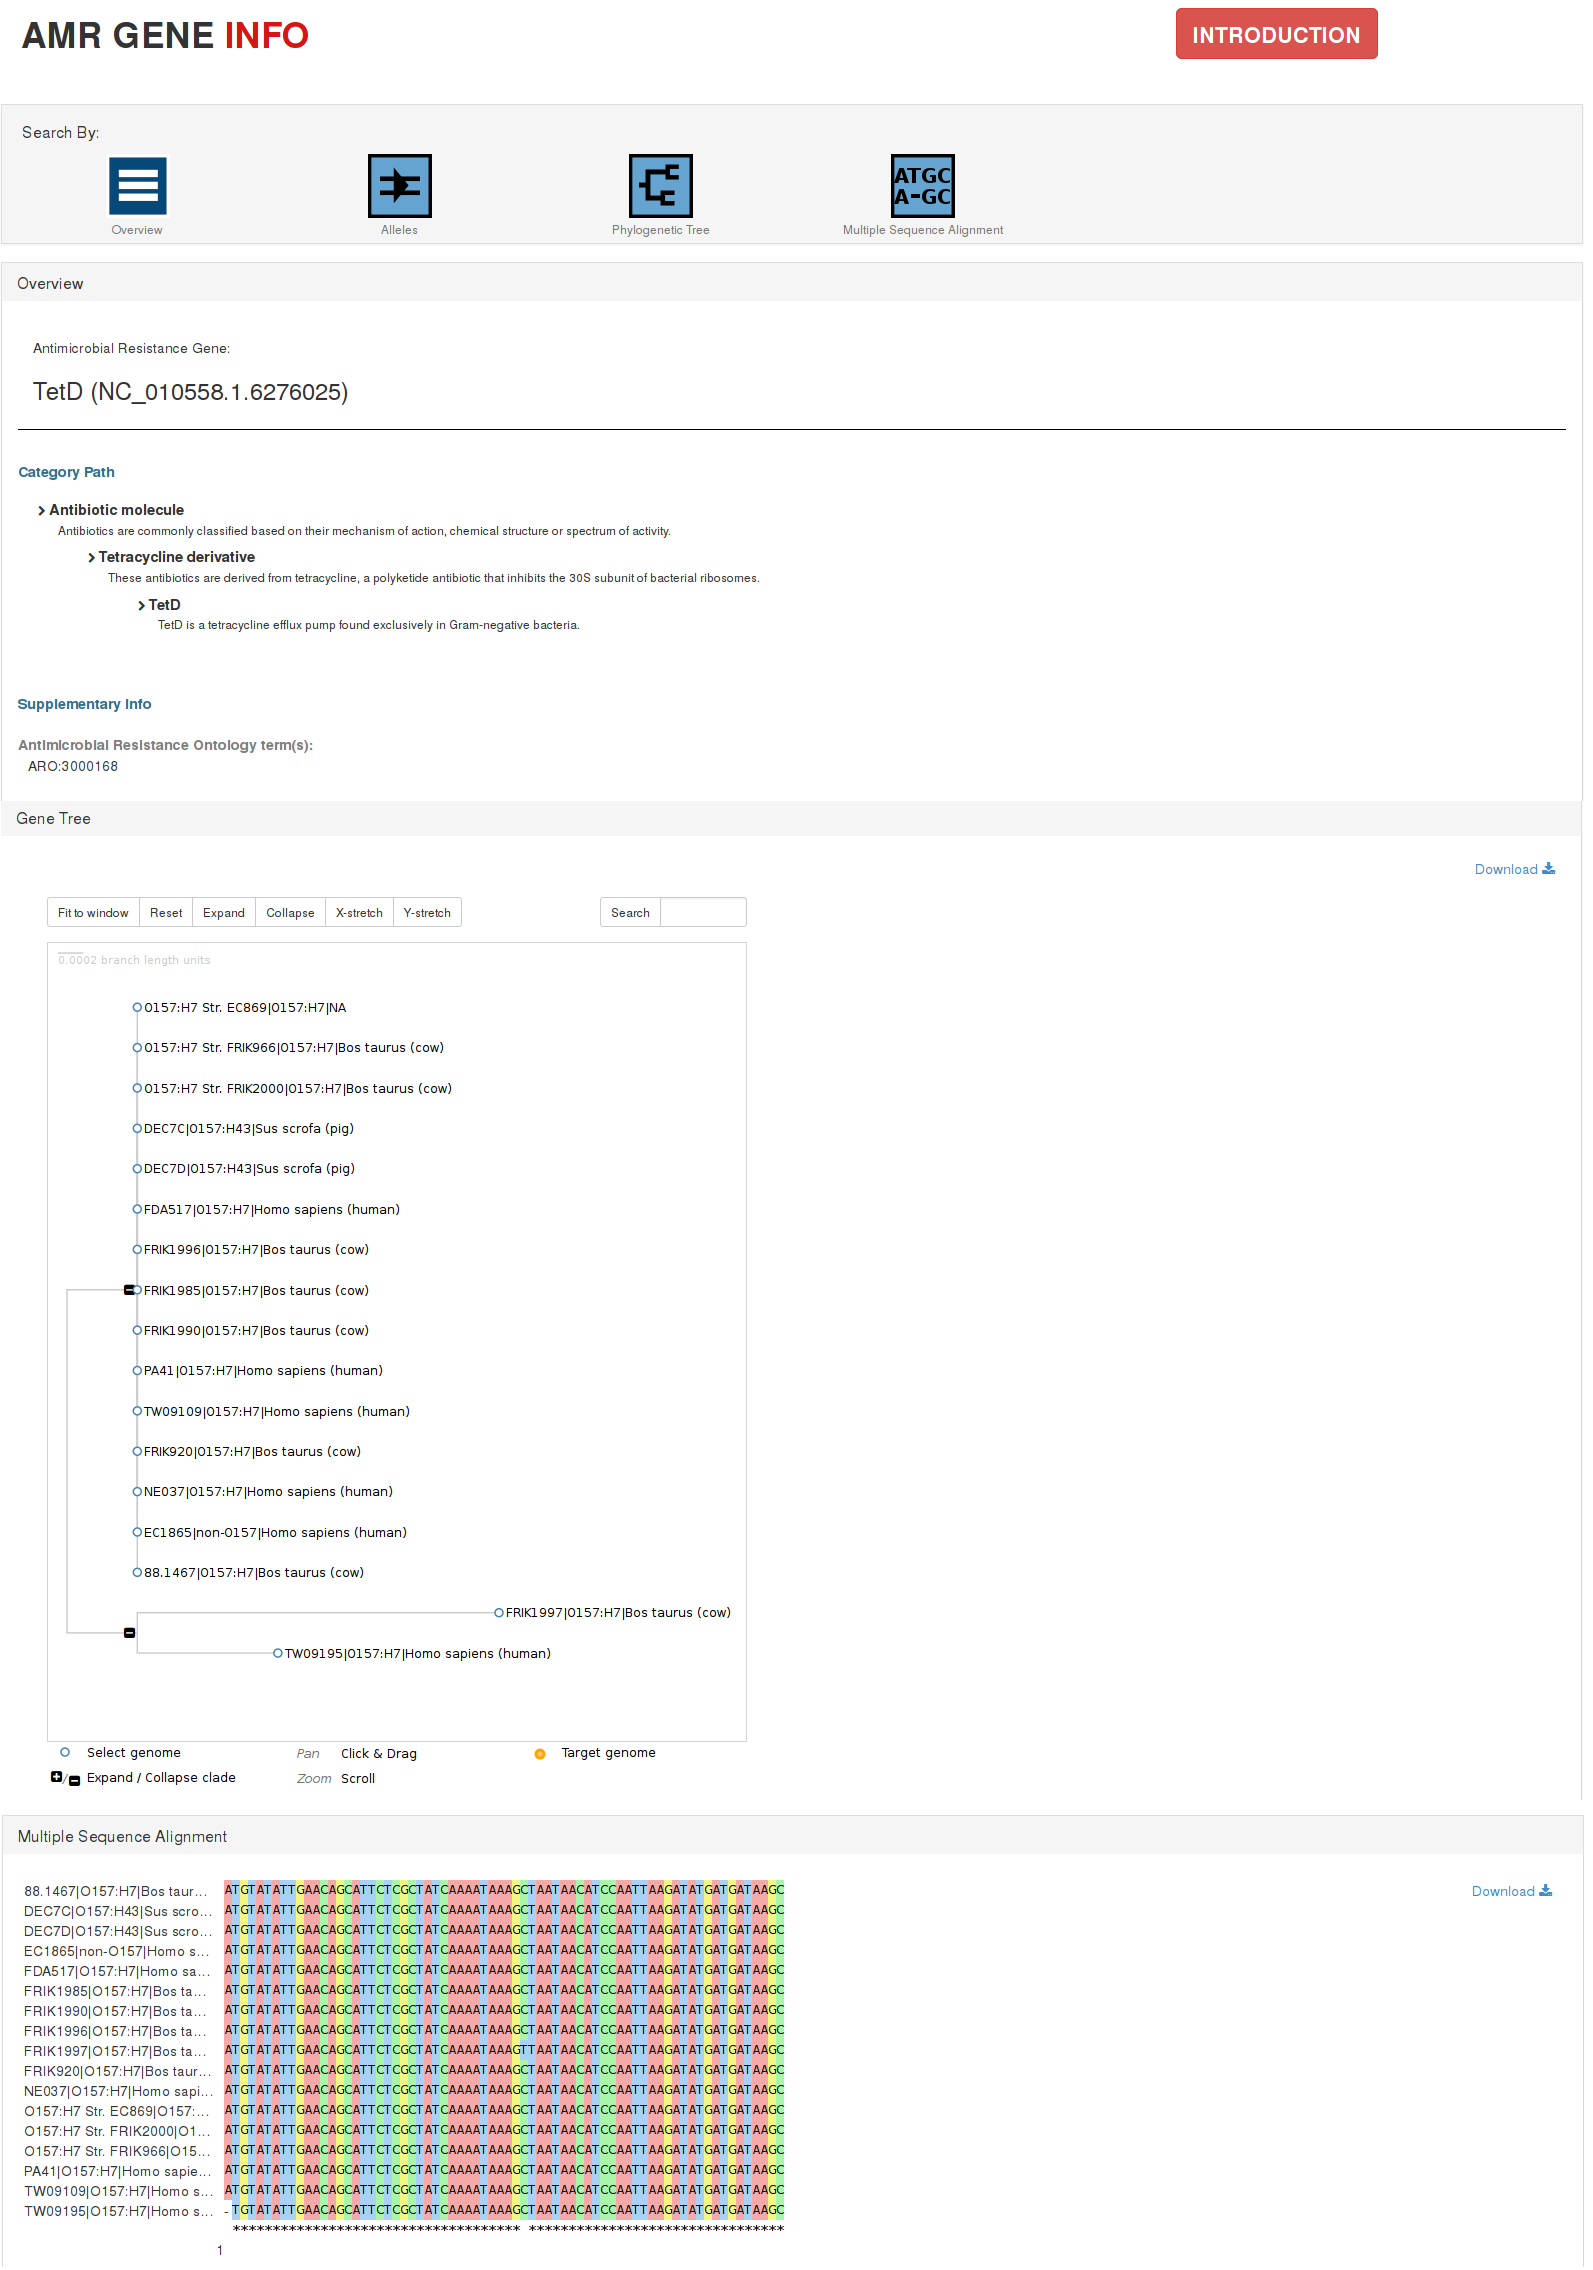
\includegraphics[width=0.7\columnwidth]{images/msa.png}
    \caption{A screen capture showing the phylogeny and accompanying multiple sequence alignment (MSA) for the gene \textit{tetD}, for all genomes in the SuperPhy database that contain a copy of the gene. Both the tree and the MSA are interactive.}
    \label{fig:msa}
\end{figure}
\end{landscape}

\newpage
\begin{figure}[h!]
  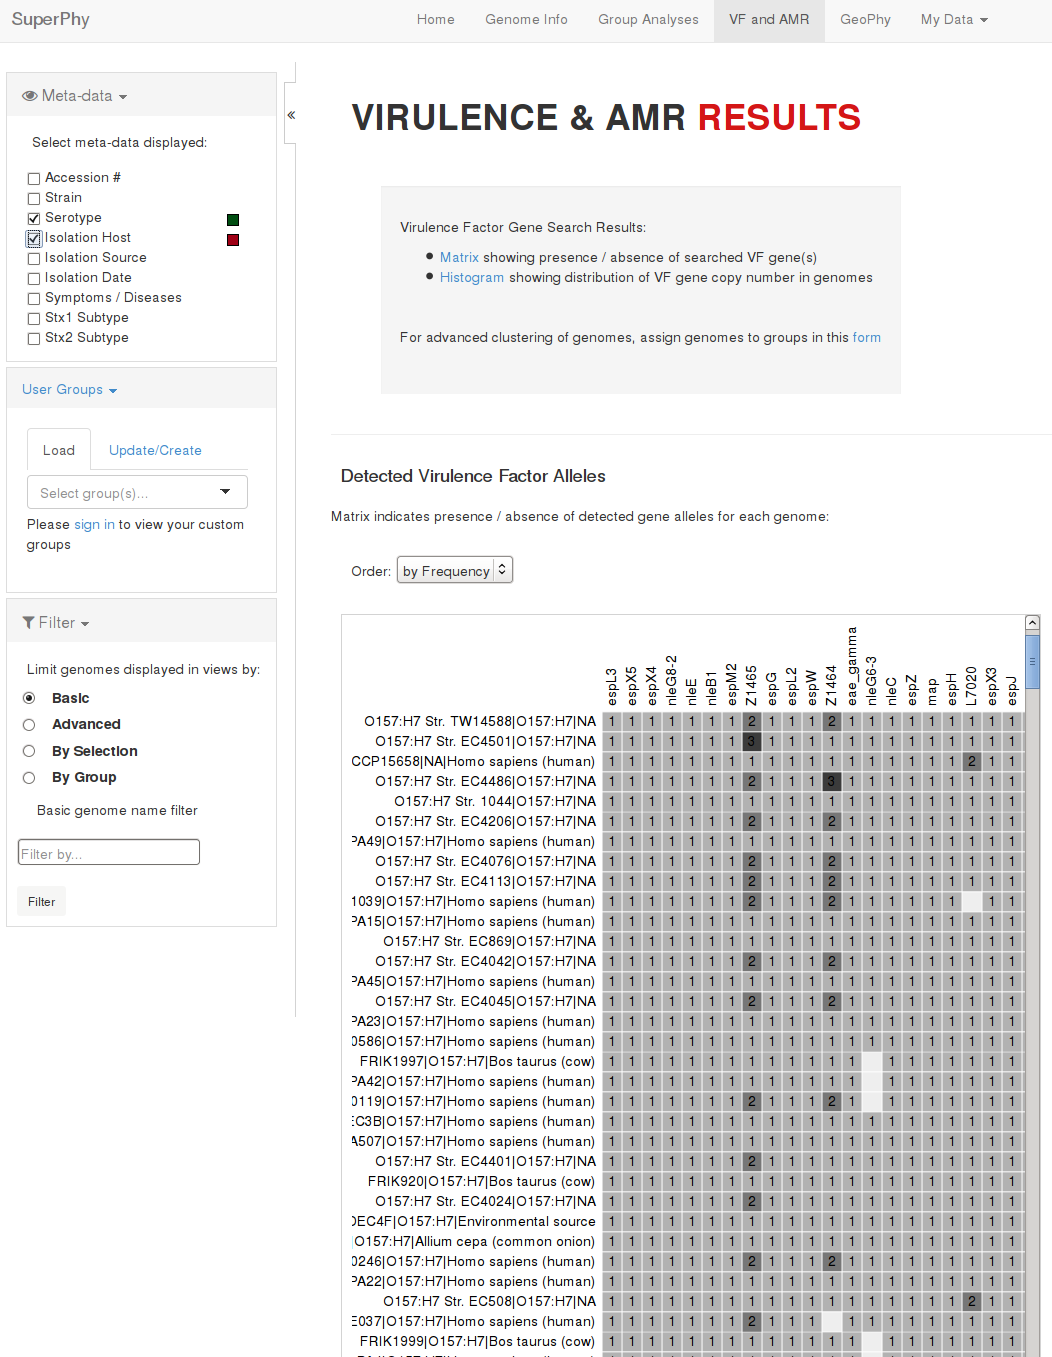
\includegraphics[width=1\columnwidth]{images/vf_output.png}
  \caption{A screen capture showing the matrix representation of all genomes that contain genes within the ontology categories `LEE-encoded TTSS effectors', `Non-LEE encoded TTSS effectors' and `Shiga-toxins', sorted by frequency of presence within a genome. The metadata categories `Serotype' and `Isolation Host' have been activated and can be seen as appended to the strain name in the row names of the matrix. The white squares indicate genomes lacking a gene, and numbered grey or black squares indicate the presence of a gene, with the number in the square indicating the number of copies of that gene in the genome.}
  \label{fig:vf_output}
\end{figure}


\newpage
\begin{figure}[h!]
   \caption{\csentence{SuperPhy tree tooltips.}}
   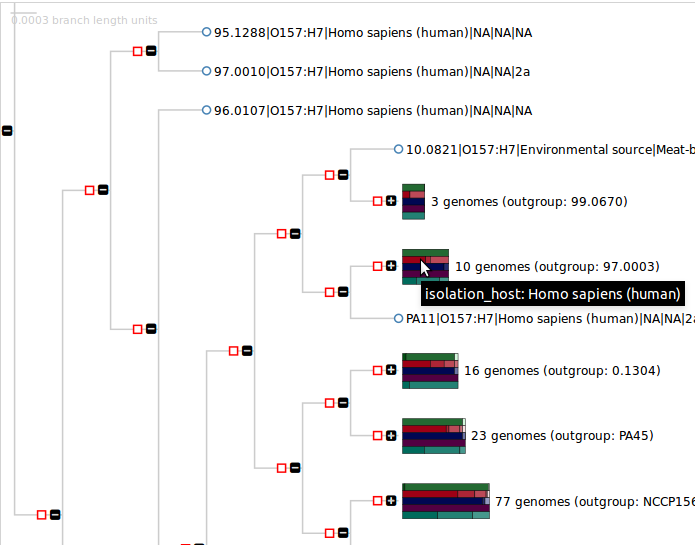
\includegraphics[width=0.9\columnwidth]{images/superphy_tree_tooltip.png}
   \label{fig:tooltip}
\end{figure}

\newpage
\begin{figure}[h!]
  \caption{Map search}
  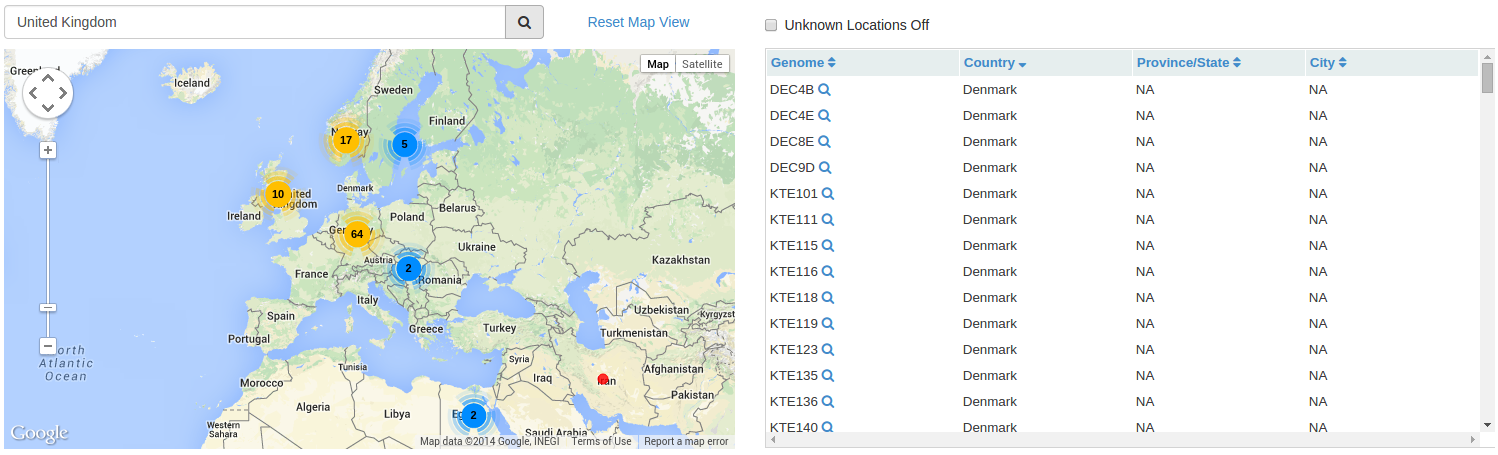
\includegraphics[width=0.9\columnwidth]{images/uk-map.png}
  \label{fig:map_search}
\end{figure}



\newpage
\begin{figure}[h!]
  \caption{Pan genome size distribution}
  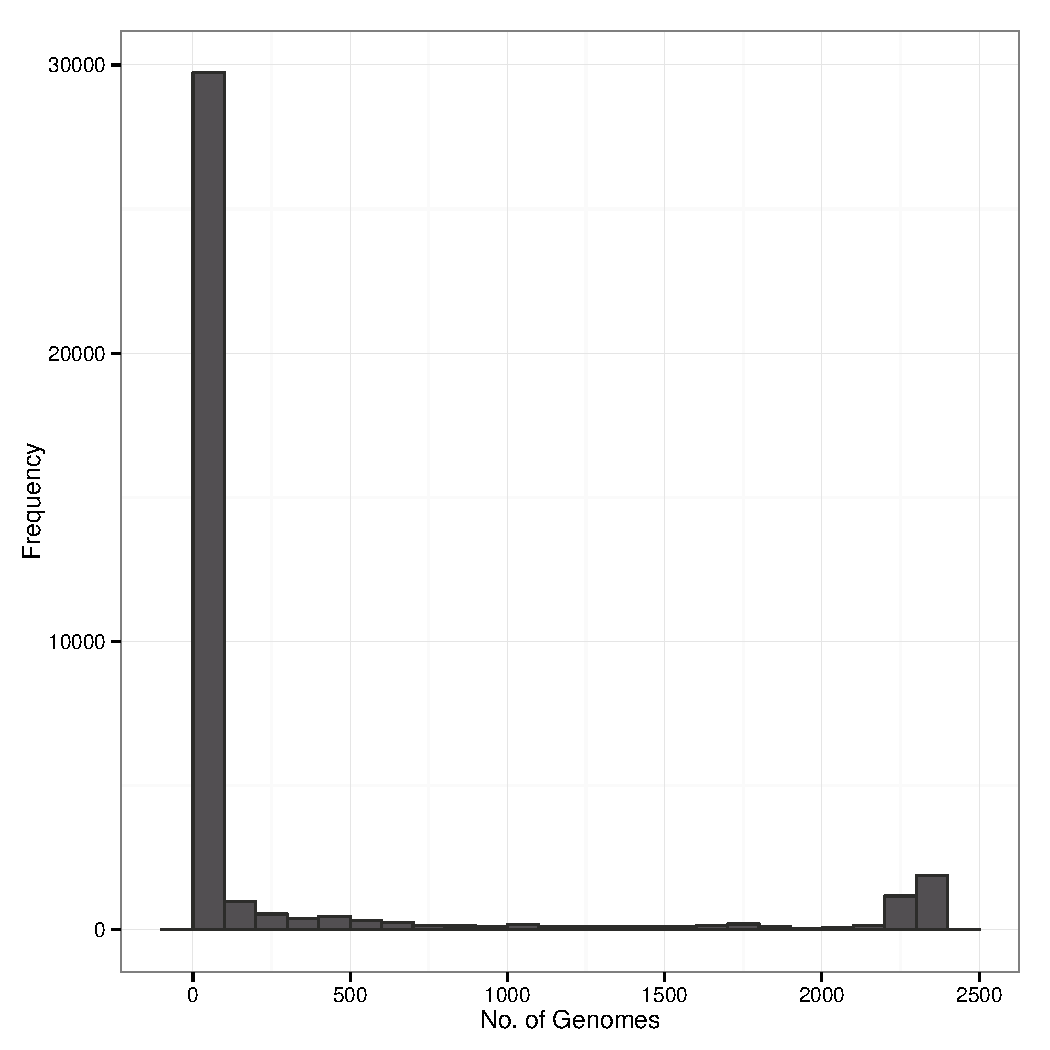
\includegraphics[width=0.9\columnwidth]{images/panGenomeSize.pdf}
  \label{fig:pan_genome_size}
\end{figure}

\newpage
\begin{figure}[h!]
  \caption{Japanese O157:H7 strains}
  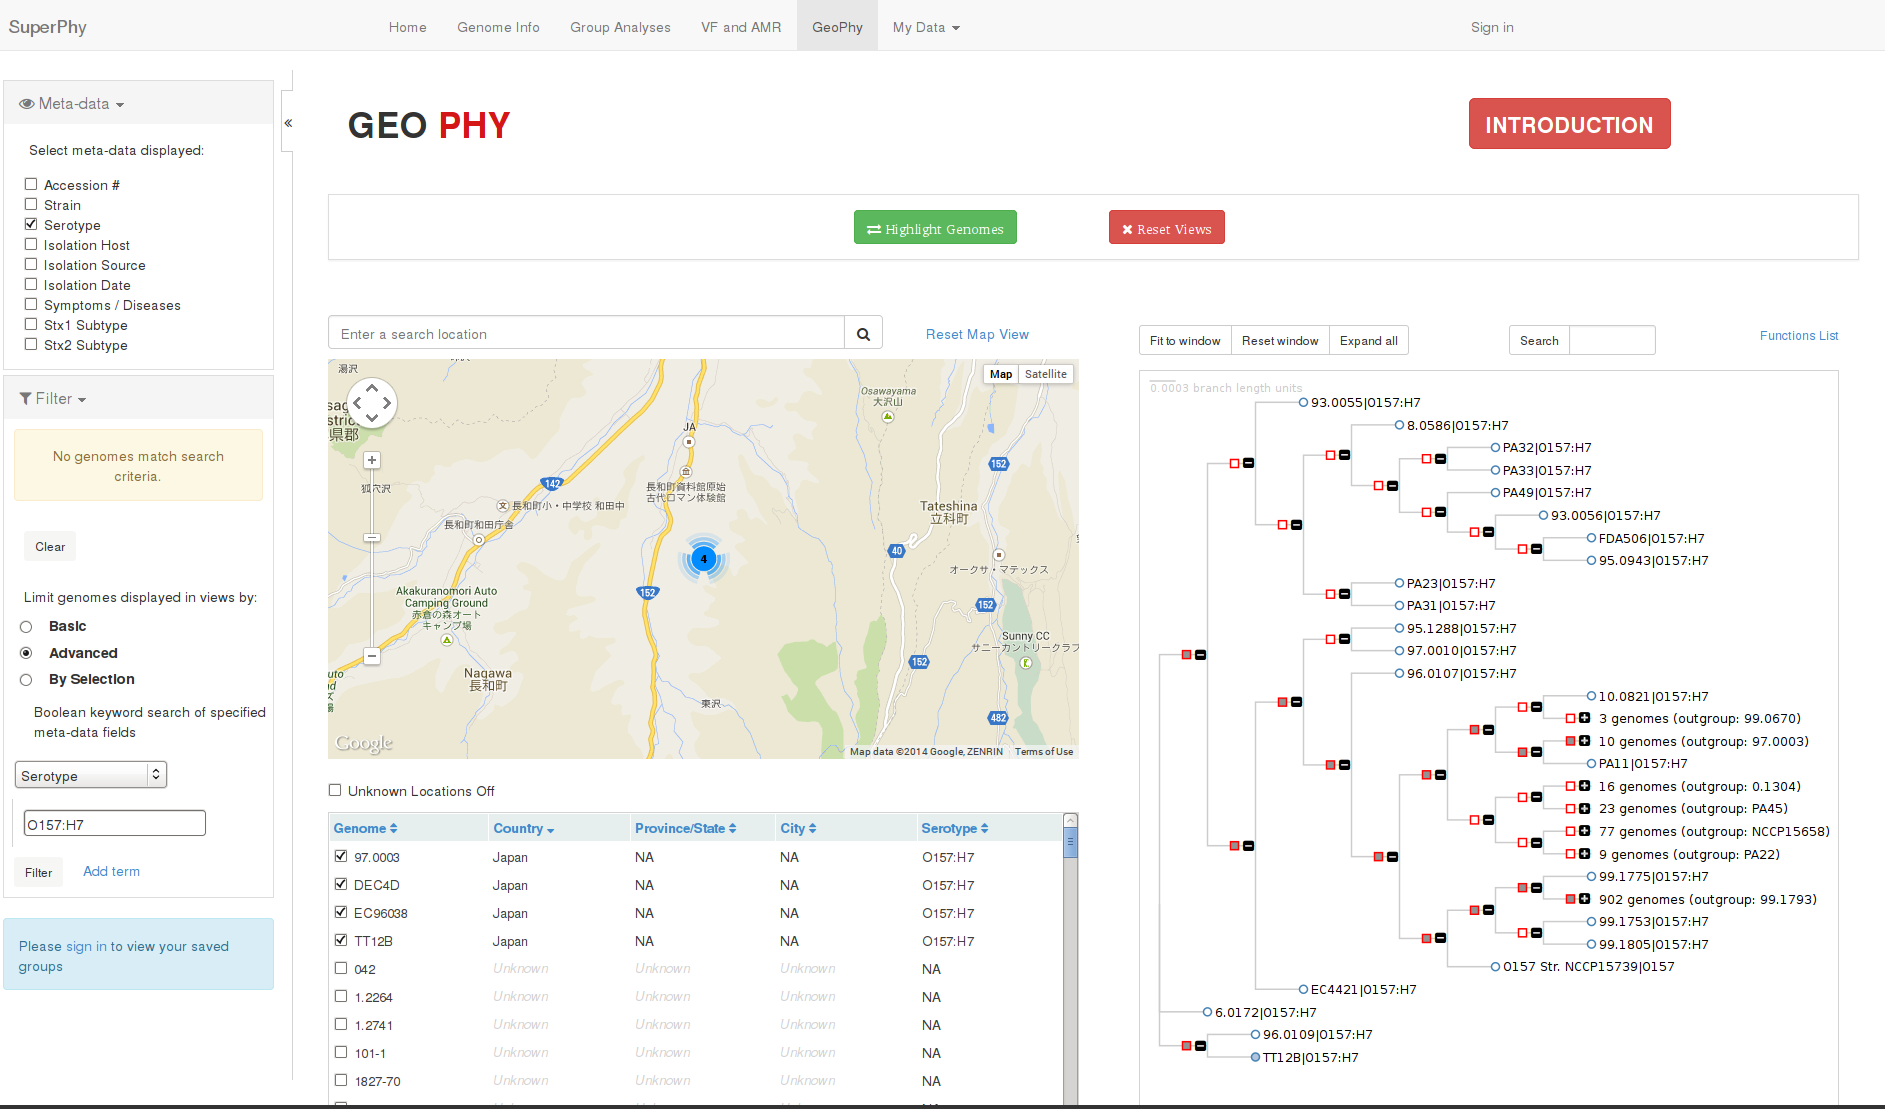
\includegraphics[width=0.9\columnwidth]{images/geophy_o157.png}
  \label{fig:geophy}
\end{figure}


%%%%%%%%%%%%%%%%%%%%%%%%%%%%%%%%%%%
%%                               %%
%% Tables                        %%
%%                               %%
%%%%%%%%%%%%%%%%%%%%%%%%%%%%%%%%%%%

%% Use of \listoftables is discouraged.
%%
\section*{Tables}
\begin{table}[h!]
\caption{The percentage of genomes that contain metadata for each of the metadata fields in the initial public data set of 1641 \textit{E. coli} in the SuperPhy database.}
\label{tab:metadata}
      \begin{tabular}{lc}
        \hline
           & Percentage\\ \hline
        Location & 60\\
        Host & 50\\
        Date of Isolation & 44\\
        Source & 35\\
        Serotype & 30\\
        Stx2 subtype & 17\\
        Stx1 subtype & 13\\
        Disease syndrome & 3\\ 
      \end{tabular}
\end{table}

%%%%%%%%%%%%%%%%%%%%%%%%%%%%%%%%%%%
%%                               %%
%% Additional Files              %%
%%                               %%
%%%%%%%%%%%%%%%%%%%%%%%%%%%%%%%%%%%

% \section*{Additional Files}
%   \subsection*{Additional file 1 --- Sample additional file title}
%     Additional file descriptions text (including details of how to
%     view the file, if it is in a non-standard format or the file extension).  This might
%     refer to a multi-page table or a figure.

%   \subsection*{Additional file 2 --- Sample additional file title}
%     Additional file descriptions text.


\end{backmatter}
\end{document}
